% !TEX root = ../CA_book.tex

\section*{2장 - 연습문제 풀이}

\subsection*{연습문제 \ref{ex-2-1}}

$z\ne0$에 대하여
\[
\dfrac{f(z) - f(0)}{z-0} - 0 = \dfrac{|z|^2-0}{z-0} = \dfrac{|z|^2}z.
\]
주어진 $\epsilon>0$에 대하여 $ \delta=\epsilon$으로 잡으면,
$0<|z-0|=|z| <\delta$일 때,
\[
\left| \dfrac{f(z) - f(0)}{z-0} - 0\right|
= \left| \dfrac{|z|^2}z \right|  = \dfrac{|z|^2}{|z|} = |z| < \delta = \epsilon.
\]
따라서 $f$는 $0$에서 복소미분가능하고 $f'(0)=0$이다.

\subsection*{연습문제 \ref{ex-2-2}}

$w_0\in \mathbb D^*$라 하자. 그러면 $\overline{w_0}\in D$이다.
$f$가 $D$에서 복소해석함수이므로, 주어진 $\epsilon>0$에 대응하는 
$\delta>0$가 존재하여,
$0<|z-\overline{w_0}| < \delta$이면 $z\in D$와
\begin{equation}\label{eq-5-17}
\left| \dfrac{f(z) - f(\overline{w_0})}{z-\overline{w_0}} - f'(\overline{w_0}) \right| < \epsilon
\end{equation}
를 만족한다.
이제 $w$를 $0<|w-w_0| <\delta$로 잡으면
\[
0< |w-w_0| = |\overline{w-w_0}| = |\overline{w} - \overline{w_0}| < \delta
\]
이 되어 $w\in D^*$이다.
또한,
\begin{align*}
\left| \dfrac{f^*(w) - f^*(w_0)}{w-w_0} - \overline{f'(\overline{w_0})} \right|
&= \left| \dfrac{\overline{f(\overline{w})} - \overline{f(\overline{w_0})}}{w-w_0} 
- \overline{f'(\overline{w_0})} \right| \\
&= \left| \overline{ \dfrac{f(\overline{w}) - f(\overline{w_0})}{w-w_0} 
- f'(\overline{w_0})} \right| \\
&= \left| \dfrac{f(\overline{w}) - f(\overline{w_0})}{w-w_0} 
- f'(\overline{w_0}) \right| < \epsilon \text{ \ (식 \eqref{eq-5-17}\을 이용하여)}
\end{align*}
이 되므로, $f^*$는 $w_0$에서 복소미분가능하며
$(f^*)'(w_0)= \overline{f'(\overline{w_0})}$이다.
$w_0\in D^*$를 임의로 선택할 수 있으므로
$f^*$는 $D^*$에서 복소미분가능함수이다.

\subsection*{연습문제 \ref{ex-2-3}}

$f$가 $z_0$에서 복소미분가능하므로,
상수 $r>0$과 함수 $h:D(z_0,r)\to \mathbb C$가 존재하여
$|z-z_0|<r$에 대하여
\[
f(z) = f(z_0) + (f'(z_0) + h(z))(z-z_0)
\]
로 쓸 수 있고
\[
\lim_{z\to z_0} h(z) = 0
\]
이다.
여기서, $D(z_0,r):= \{ z\in \mathbb C \,:\, |z-z_0| < r\} \subset D$이다.

$D(z_0,r'):= \{ z\in \mathbb C \,:\, |z-z_0| < r'\} \subset D(z_0,r) \subset D$과
$|h(z)|<1$이 되도록 $r'<r$을 잡자.
이제 주어진 $\epsilon>0$에 대하여
\[
\delta = \min\left\{ \dfrac\epsilon{|f'(z_0)|+1}, r' \right\}
\]
로 선택하면, $0<|z-z_0|<\delta$일 때, 
$z\in D(z_0, r')$이고,
\begin{align*}
|f(z) - f(z_0)| = |f'(z_0) + h(z)||z-z_0|
&\le ( |f'(z_0)|+|h(z)|)\dfrac{\epsilon}{ |f'(z_0)|+1} \\
&< ( |f'(z_0)|+1)  \dfrac{\epsilon}{|f'(z_0)|+1} = \epsilon.
\end{align*}
따라서 $f$는 $z_0$에서 연속이다.

\subsection*{연습문제 \ref{ex-2-4}}

$f,g:U\to \mathbb C$가 $z_0\in U$에서 복소미분가능함을 이용하면,
보조정리 \ref{lem-2-1}\로부터
$r>0$과 $h_f, h_g: D(z_0,r) \to \mathbb C$가 존재하여
(단, $D(z_0,r):= \{ z\in \mathbb C \,:\, |z-z_0| < r\}$)

$|z-z_0|<r$이면,
\begin{align}
f(z) & = f(z_0) + (f'(z_0) +h_f(z))(z-z_0), \label{eq-5-18} \\
g(z) & = g(z_0) + (g'(z_0) +h_g(z))(z-z_0), \label{eq-5-19}
\end{align}
와 $\Lim_{z\to z_0} h_f(z)  = 0 = \Lim_{z\to z_0} h_g(z)$를 만족한다.
\begin{itemize}
\item[(1)] 식 \eqref{eq-5-18}\과 \eqref{eq-5-19}\를 더하면,
$|z-z_0|<r$에 대하여
\[
(f+g)(z) = (f+g)(z_0) + \left( f'(z_0) + g'(z_0) + h_{f+g}(z) \right)(z-z_0)
\]
를 만족한다. 단, $D(z_0,r)$에서 $h_{f+g} (z) := h_f(z) + h_g(z)$로 정의한다.
또한,
\[
\lim_{z\to z_0} h_{f+g}(z) = \lim_{z\to z_0} ( h_f(z) + h_g(z) )
= \lim_{z\to z_0} h_f(z) + \lim_{z\to z_0} h_g(z) = 0+0 = 0.
\]
보조정리 \ref{lem-2-1}에 의하여
$f+g$는 복소미분가능하며 $(f+g)'(z_0) = f'(z_0) + g'(z_0)$이다.
\item[(2)] 식 \eqref{eq-5-18}에 $\alpha$를 곱하면,
$|z-z_0|<r$에 대하여
\[
(\alpha \cdot f)(z) = (\alpha \cdot f)(z_0) + \left(
\alpha\cdot f'(z_0) + h_{\alpha\cdot f}(z) \right) (z-z_0),
\]
단, $D(z_0,r)$에서 $h_{\alpha\cdot f}(z) := \alpha \cdot f(z)$이다.
또한,
\[
\lim_{z\to z_0} h_{\alpha\cdot f}(z) = \lim_{z\to z_0} (\alpha\cdot h_f(z))
= \alpha \cdot \lim_{z\to z_0} h_f(z) = \alpha\cdot 0 = 0.
\]
보조정리 \ref{lem-2-1}에 의하여
$\alpha \cdot f$는 복소미분가능하며 $(\alpha\cdot f)'(z_0) =\alpha\cdot f'(z_0)$이다.

\item[(3)] 식 \eqref{eq-5-18}\과 \eqref{eq-5-19}\를 곱하면,
$|z-z_0|<r$에 대하여
\[
(fg)(z) = (fg)(z_0) + \left( f'(z_0)g(z_0) + f(z_0)g'(z_0) + h_{fg}(z) \right) (z-z_0),
\]
단, $D(z_0,r)$에서
\[
h_{fg}(z):= f(z_0)h_g(z) + g(z_0)h_f(z) + (z-z_0)(f'(z_0)+h_f(z))(g'(z_0)+h_g(z))
\]
또한,
\[
\lim_{z\to z_0} h_{fg}(z) = f(z_0)\cdot0 + g(z_0)\cdot 0 
+ 0\cdot (f'(z_0)+0)\cdot(g'(z_0)+0)=0
\]
이므로 $fg$는 $z_0$에서 복소미분가능하며
\[
(fg)'(z) = f'(z_0)g(z_0) + f(z_0)g'(z_0).
\]
\end{itemize}

\subsection*{연습문제 \ref{ex-2-5}}

$\Hol(\mathbb D)$가 $d$차의 유한차원이라고 하자.
그러면 $d+1$개의 벡터 $1,z, z^2, \ldots, z^d\in \Hol(\mathbb  D)$는
일차종속이다. 따라서 모두 $0$은 아닌 $\alpha_0, \ldots, \alpha_d$가 존재하여
\[
\alpha_0\cdot 1 + \alpha_1\cdot z + \cdots + \alpha_d \cdot z^d = 0
\quad(z\in \mathbb D)
\]
을 만족한다.
$k\in \{0, 1, \ldots, d\}$를 $\alpha_k \ne 0$인 가장 작은 값이라 하자.
그러면, $k$번 미분한 값을 $0\in \mathbb D$에서 계산하면
\[
0 + \alpha_k \cdot k! + 0 = 0
\]
이므로 $\alpha_k=0$이 되어 모순이다.

\subsection*{연습문제 \ref{ex-2-6}}

$z_0\in U$라 하자. $f$는 $z_0$에서 복소미분가능하므로
$r>0$과 $D(z_0,r) := \{ z\in \mathbb C\,:\, |z-z_0|<r\} \subset U$에 정의된
복소함수 $h$가 존재하여
\[
f(z) = f(z_0) + (f'(z_0) +h(z))(z-z_0),
\quad z\in D(z_0,r)
\]
과
\begin{equation}\label{eq-5-20}
\lim_{z\to z_0} h(z)=0
\end{equation}
을 만족한다.
$g:=1/f$라 하면,
\[
\dfrac1{g(z)} = \dfrac1{g(z_0)} + (f'(z_0) +h(z))(z-z_0)
\]
이므로 $g(z_0) = g(z) + (f'(z_0)+h(z))g(z_0)g(z)\cdot(z-z_0)$.
정리하면
\begin{align*}
g(z) &= g(z_0) + (-f'(z_0)g(z_0)g(z) - h(z)g(z_0)g(z)))\cdot(z-z_0) \\
&= g(z_0) + \left( - \dfrac{f'(z_0)}{(f(z_0))^2} + \dfrac{f'(z_0)}{(f(z_0))^2}
- \dfrac{f'(z_0)}{f(z_0)f(z)} - \dfrac{h(z)}{f(z_0)f(z)} \right) (z-z_0) \\
&= g(z_0) + \left( - \dfrac{f'(z_0)}{(f(z_0))^2} + \varphi(z) \right)\cdot(z-z_0),
\end{align*}
$z\in D(z_0,r)$에서
\[
\varphi(z):= \dfrac{f'(z_0)}{(f(z_0))^2}
- \dfrac{f'(z_0)}{f(z_0)f(z)} - \dfrac{h(z)}{f(z_0)f(z)}.
\]
$z_0$에서 $f$의 연속성과 식 \eqref{eq-5-20}\로부터
\[
\lim_{z\to z_0} \varphi(z) = \cancel{\dfrac{f'(z_0)}{(f(z_0))^2}}
- \cancel{\dfrac{f'(z_0)}{f(z_0)f(z_0)}} - \dfrac{0}{f(z_0)f(z_0)} = 0.
\]
따라서 $g$가 $z_0$에서 복소미분가능하며
\[
g'(z_0) = - \dfrac{f'(z_0)}{(f(z_0))^2}.
\]

\subsection*{연습문제 \ref{ex-2-7}}

$m\ge0$인 경우는 이미 증명했으므로, 
$m= -n$ ($n\in \mathbb N$)인 경우를 생각하자.
$f(z):=z^n$ ($z\in \mathbb C\setminus \{0\}$)에  대하여 함수
\[
z\mapsto z^m = z^{-n} = \dfrac1{z^n} = \dfrac1{f(z)}
\]
는 복소해석함수이고 $\mathbb C\setminus \{0\}$에서 함수값이
$0$은 아니므로
$1/f$도 복소해석함수이고, 미분은
\[
\left(\dfrac1f\right)'(z) = - \dfrac{f'(z)}{(f(z))^2} = - \dfrac{nz^{n-1}}{(z^n)^2}
= -n \dfrac1{z^{n+1}} = m \cdot \dfrac1{z^{-m+1}} = mz^{m-1}
\]
이 되어 증명이 끝난다.

\subsection*{연습문제 \ref{ex-2-8}}

$f: \mathbb D \to \mathbb C$를 
\[
f(z) = -\dfrac{1+z}{1-z},\quad z\in \mathbb D
\]
로 정의하고, $f: \mathbb C \to \mathbb C$를 $g(z)= \exp z$로 정의하자.
그러면, $f(\mathbb D) \subset \mathbb C = D_g$.
따라서 $g\circ f$는 $\mathbb D$에서 복소해석함수이고,
\begin{align*}
(g\circ g)'(z) &= g'(f(z))\cdot f'(z) 
= \exp\left( - \dfrac{1+z}{1-z}\right) \cdot \dfrac d{dz}\left( - \dfrac{1+z}{1-z}\right) \\
&= \exp\left( - \dfrac{1+z}{1-z}\right)\cdot \left(
-(1+z)\dfrac d{dz} \left(\dfrac1{1-z}\right) - \dfrac1{1-z}\dfrac d {dz}(1+z)\right) \\
&= \exp\left( - \dfrac{1+z}{1-z}\right) \cdot \left(
-\dfrac{1+z}{(1-z)^2} - \dfrac1{1-z} \right) \\
&= - \dfrac2{(1-z)^2} \exp\left( - \dfrac{1+z}{1-z}\right).
\end{align*}
따라서, $z\in\mathbb D$에 대하여,
$\dfrac d{dz} \left( \exp\left( - \dfrac{1+z}{1-z}\right) \right)
=  - \dfrac2{(1-z)^2} \exp\left( - \dfrac{1+z}{1-z}\right)$.

\subsection*{연습문제 \ref{ex-2-9}}

$z = x+iy$ ($x,y\in\mathbb R$)라 하면,
$|z|^2 = x^2+y^2$.
따라서, $u, v$를 각각 $|z|^2$의 실수부와 허수부라 하면,
$u=x^2+y^2$, $v=0$이다. 따라서,
\begin{align*}
\dfrac{\partial u}{\partial x} &=2x, \quad \dfrac{\partial v}{\partial y} = 0, \\
\dfrac{\partial u}{\partial y} &=2y, \quad \dfrac{\partial v}{\partial x} = 0.
\end{align*}
$z\ne0$이므로, $x$ 또는 $y$중 하나는 $0$이 아니다.
즉, 코시-리만 방정식 중 적어도 하나는 만족되지 않는다.
\begin{align*}
\left( \dfrac{\partial u}{\partial x} = \right) 2x &\ne 0 
\left( = \dfrac{\partial v}{\partial y} \right) \text{ 또는} \\
\left( \dfrac{\partial u}{\partial y} = \right) 2y &\ne 0 
\left( = - \dfrac{\partial v}{\partial x} \right).
\end{align*}
결론적으로 $|z|^2$은 $0$이 아닌 점에서 미분이 불가능하다.

\subsection*{연습문제 \ref{ex-2-10}}

$z = x+iy$ ($x,y\in\mathbb R$)라 하면,
\begin{align*}
z^3 &= (x+iy)^3 = x^3 + 3x^2(iy) + 3x(iy)^2 + (iy)^3 \\
&= x^3 - 3xy^2 + i(3x^2y-y^3).
\end{align*}

$u$, $v$를 각각 $z^3$의 실수부와 허수부라 하면,
\begin{align*}
u(x,y) &= x^3 -3xy^2, \\
v(x,y) &= 3x^2y - y^3.
\end{align*}

$u$, $v$는 연속미분가능하고 (즉, $u,v\in C^1$)
\begin{align*}
\dfrac{\partial u}{\partial x} &= 3x^2 -2y^2 = \dfrac{\partial v}{\partial y} \text{ 이고}, \\
\dfrac{\partial u}{\partial y} &= -6xy = - \dfrac{\partial v}{\partial x}.
\end{align*}
즉, $\mathbb R^2$의 모든 점에서 코시-리만 방정식을 만족하므로,
$z\mapsto z^3$은 전해석함수이다.

\subsection*{연습문제 \ref{ex-2-11}}

$z = x+iy$ ($x,y\in\mathbb R$)라 하면,
$\Re(z) = \Re(x+iy) = x$.
따라서, $u, v$를 각각 $\Re(z)$의 실수부와 허수부라 하면,
\begin{align*}
u & =x, \\
v &=0.
\end{align*}
따라서, 모든 $(x,y) \in \mathbb R^2$에서
\[
\dfrac{\partial u}{\partial x}  = 1 \ne 0 =  \dfrac{\partial v}{\partial y}.
\]
즉, 코시-리만 방정식은 $\mathbb R^2$의 어떤 점에서도 만족되지 않는다.
결론적으로 $\mathbb C$의 모든 점에서 $\Re(z)$는 복소미분가능하지 않다.

\subsection*{연습문제 \ref{ex-2-12}}

$u$, $v$를 각각 $f$의 실수부와 허수부라 하자. 
그러면, $v=0$이고,
\[
\dfrac{\partial u}{\partial x} = \dfrac{\partial v}{\partial y} = 0
\text{ 이고 }
\dfrac{\partial u}{\partial y} = - \dfrac{\partial v}{\partial x} = 0.
\]
따라서 $(x_0,y_0)\in D$과 $(x, y_0)\in D$를 잇는 직선이  $D$ 내부에 있을 때, 이 직선을 따라 적분하면
\[
u(x,y_0) - u(x_0,y_0) = \int_{x_0}^x \dfrac{\partial u}{\partial x}(\xi, y_0) d\xi = 0.
\]
같은 방법으로 
 $(x_0,y_0)\in D$과 $(x_0, y)\in D$를 잇는 직선이  $D$ 내부에 있을 때, 
\[
u(x_0,y) - u(x_0,y_0) = \int_{y_0}^y \dfrac{\partial u}{\partial y}(x_0, \eta) d\eta = 0.
\]
즉, $D$의 내부에서 수평선 또는 수직선을 따라 움직이는 동안 $u$의 값은 변하지 않는다.
그런데 $D$가 경로연결 집합이므로 $u$는 $D$에서 상수이다.
(왜냐하면, $D$에 속하는 임의의  두점은 계단형 경로로 연결할 수 있기 때문이다.)
따라서 $f=u+i0 = u$는 $D$에서 상수이다.

\subsection*{연습문제 \ref{ex-2-13}}

$u$, $v$가 각각 $f$의 실수부와 허수부라고 하자.
$f'(z) = \dfrac{\partial u}{\partial x} + i \dfrac{\partial v}{\partial x} = 0$이면
$D$에서
\[
\dfrac{\partial u}{\partial x} = \dfrac{\partial v}{\partial x} = 0
\]
이고 코시-리만 방정식을 이용하면
\[
\dfrac{\partial u}{\partial y} \left( = - \dfrac{\partial v}{\partial x} \right) =0,
\dfrac{\partial v}{\partial y} \left( = \dfrac{\partial u}{\partial x} \right) =0.
\]
따라서   $(x_0,y_0)\in D$과 $(x, y_0)\in D$를 잇는 직선이  $D$ 내부에 있을 때, 이 직선을 따라 적분하면
\[
u(x,y_0) - u(x_0,y_0) = \int_{x_0}^x \dfrac{\partial u}{\partial x}(\xi, y_0) d\xi = 0.
\]
같은 방법으로 
 $(x_0,y_0)\in D$과 $(x_0, y)\in D$를 잇는 직선이  $D$ 내부에 있을 때, 
\[
u(x_0,y) - u(x_0,y_0) = \int_{y_0}^y \dfrac{\partial u}{\partial y}(x_0, \eta) d\eta = 0.
\]
연습문제 \ref{ex-2-13}에서와 같이 
$D$의 내부에서 수평선 또는 수직선을 따라 움직이는 동안 $u$의 값은 변하지 않는다.
그런데 $D$가 경로연결 집합이므로 $u$는 $D$에서 상수이다.
(왜냐하면, $D$에 속하는 임의의  두점은 계단형 경로로 연결할 수 있기 때문이다.)
따라서 $f=u+iv$는 $D$에서 상수이다.

\subsection*{연습문제 \ref{ex-2-14}}

연쇄법칙으로부터 다음 관계식을 얻는다.
\[
\dfrac{\partial u}{\partial x} (x,y) = h'(v(x,y))\dfrac{\partial v}{\partial x}  (x,y),
\quad
\dfrac{\partial u}{\partial y} (x,y) = h'(v(x,y))\dfrac{\partial v}{\partial y}  (x,y).
\]
코시-리만 방정식을 적용하면
\begin{align*}
\dfrac{\partial u}{\partial y} (x,y) 
&= h'(v(x,y))\dfrac{\partial v}{\partial y}  (x,y)
= h'(v(x,y))\dfrac{\partial u}{\partial x}  (x,y) \\
&= h'(v(x,y))\cdot\left( h'(v(x,y))\dfrac{\partial v}{\partial x}(x,y) \right) 
= (h'(v(x,y))^2\cdot \dfrac{\partial v}{\partial x}(x,y) \\
&= - (h'(v(x,y))^2\cdot \dfrac{\partial u}{\partial y}(x,y)
\end{align*}
이므로
$(1+(h'(v(x,y)))^2) \dfrac{\partial u}{\partial y}(x,y) = 0$.
$(1+(h'(v(x,y)))^2)\ge0 >1$로부터
\[
\dfrac{\partial u}{\partial y}(x,y) = 0.
\]
코시-리만 방정식을 다시 적용하면
\[
\dfrac{\partial v}{\partial x}(x,y) = - \dfrac{\partial u}{\partial y}(x,y) = 0
\]
도 얻으며, 이로부터
\[
\dfrac{\partial u}{\partial x} (x,y) = h'(v(x,y))\dfrac{\partial v}{\partial x}  (x,y)
= h'(v(x,y))\cdot 0 = 0
\]
이고 코시-리만 방정식을 한번 더 적용하면,
\[
\dfrac{\partial v}{\partial y}(x,y) = \dfrac{\partial u}{\partial x}(x,y) = 0.
\]
이제 모든 편도함수가 $0$이 되므로,
$u$는 수평, 수직방향을 따라 상수이다.
$D$가 영역이므로, 경로연결 집합이고, 임의의 두 점이 계단형 경로로 연결가능하다.
따라서 $u$는 $D$에서 상수함수이다.
같은 방법이로, $v$도 $D$에서 상수함수이며,
$f=u+iv$도 상수함수가 된다.

\subsection*{연습문제 \ref{ex-2-15}}

($\Leftarrow$)

$k=2$라고 하면,
\[
f(z) = x^2-y^2 + 2xyi = x^2 + (iy)^2 + 2x(iy) = (x+iy)^2 = z^2.
\]
예제 \ref{example-2-1}에 의하여 $f$는 전해석함수이다.

\noindent($\Rightarrow$)

이제 $f$가 전해석함수라고  가정하자.
그러면 모든 점에서 코시-리만 방정식을 만족해야 하므로, 모든 $x, y\in \mathbb R$에 대하여
\[
\dfrac{\partial u}{\partial x} = 2x = kx = \dfrac{\partial v}{\partial y}.
\]
특히 $x=1$로 잡으면, $k=2$을 얻는다.

\subsection*{연습문제 \ref{ex-2-16}}

$z-z_0$의 길이가 $|z_0|\tan(d\theta) \approx |z_0| d\theta$이므로
$z^n-z_0^n$의 길이는 $|z_0|^n\tan(nd\theta) \approx |z_0|^nnd\theta$이다.
따라서 국소적으로 $z\mapsto z^n$에 의한 확대비율은
\[
 \dfrac{|z^n-z_0^n|}{|z-z_0|} \approx \dfrac{|z_0|^n nd\theta}{|z_0|d\theta}
 = n|z_0|^{n-1}
\]
이고, 그림에 따르면 반시계방향으로 $(n-1)\theta$만큼 회전한 변환이다.
\begin{align*}
f'(z_0) &= n|z_0|^{n-1} ( \cos((n-1)\theta) + i\sin((n-1)\theta) ) \\
&= n(|z_0|(\cos\theta + i\sin\theta))^{n-1} = nz_0^{n-1}.
\end{align*}
결론적으로, 모든 $\mathbb C$에 대하여 $\dfrac d{dz} z^n = nz^{n-1}$.

\begin{figure*}[h!]
\begin{center}
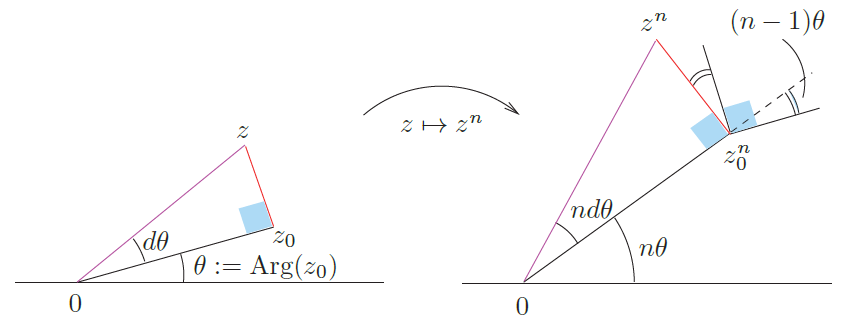
\includegraphics[width=0.8\textwidth]{./Solution/figs/fig-s-0-6}
\end{center}
%\caption{$\left\{ z \in\mathbb C \,:\, z\ne0, \dfrac\pi4 < |\Arg(z)| < \dfrac\pi3 \right\}$}
%\label{fig-5-14}
\end{figure*}

\subsection*{연습문제 \ref{ex-2-17}}

\begin{figure}[h!]
\begin{center}
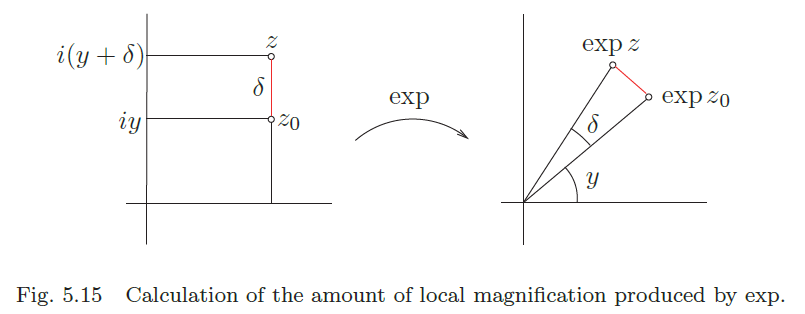
\includegraphics[width=0.7\textwidth]{./Solution/figs/fig-5-15}
\end{center}
\caption{$\exp$ 함수에 의한 국소적인 확대비율
}
\label{fig-5-15}
\end{figure}

그림 \ref{fig-5-15}에서
확대비율은
\[
\dfrac{e^x\cdot \delta}{\delta} = e^x
\]
이다. 
아래 그림과 같이 반시계방향으로  $y$만큼 회전하는 변환이므로
$z_0$에서 복소미분은 $e^x(\cos y + i\sin y) = \exp(x+iy)$,
즉, $\exp' z = \exp z$이다.

\begin{figure*}[h!]
\begin{center}
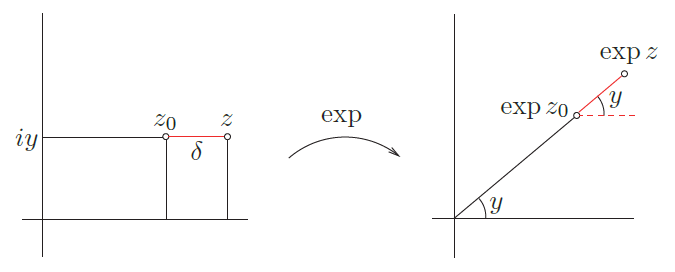
\includegraphics[width=0.7\textwidth]{./Solution/figs/fig-s-0-7}
\end{center}
%\caption{$\left\{ z \in\mathbb C \,:\, z\ne0, \dfrac\pi4 < |\Arg(z)| < \dfrac\pi3 \right\}$}
%\label{fig-5-14}
\end{figure*}

\subsection*{연습문제 \ref{ex-2-18}}

$z_0 \in \mathbb C$에 대하여,
$z_0$를 기울기 $1$인 직선을 따라 $\delta$만큼 움직인 점을 $z$라고 하자.
유사한 방법으로 $z_0$를 수평선을 따라 왼쪽으로 $\delta$만큼 이동한 점을 $\tilde z$라고 하자.
실수부를 취하는 함수 $\Re(\cdot)$가 $z_0$에서 미분가능하다고 가정하자.
그림 \ref{fig-5-16}에서 $z$ 와 $\tilde z$를 $\Re(\cdot)$로 보낸 점을 보면 
국소적으로 각각 $45^\circ$와 $0^\circ$ 회전한 것으로 다른 회전량을 갖는다.
이는 일어날 수 없는 경우로 복소미분가능하다는 가정에 모순이다.
$z_0\in \mathbb C$의 선택을 임의로  할 수 있으므로
이 함수는 모든 점에서 복소미분불가능하다.


\begin{figure}[h!]
\begin{center}
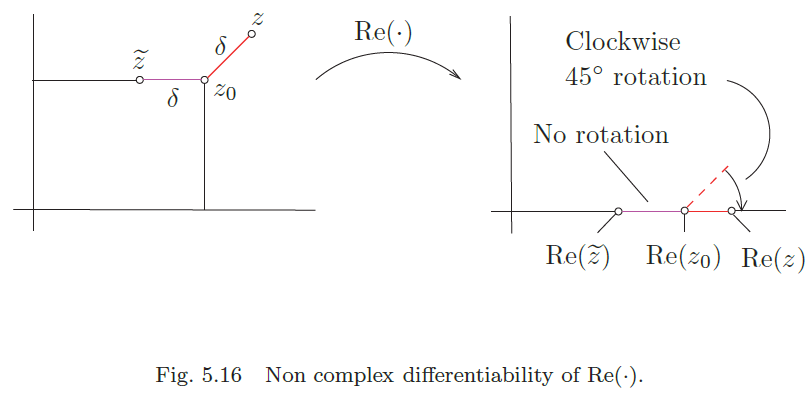
\includegraphics[width=0.7\textwidth]{./Solution/figs/fig-5-16}
\end{center}
\caption{함수 $\Re(\cdot)$의 복소미분 불가능성}
\label{fig-5-16}
\end{figure}

\subsection*{연습문제 \ref{ex-2-19}}

$u,v\in C^2$인 $f=u+iv$는 두번 연속미분가능하므로
\begin{align*}
4\dfrac\partial{\partial z}\dfrac\partial{\partial \bar z}f
&= \cancel{4}\cdot \dfrac1{\cancel{2}} \left(\dfrac\partial{\partial x} - i \dfrac\partial{\partial y} \right)
\cdot\dfrac1{\cancel{2}} \left( \dfrac{\partial u}{\partial x} + i \dfrac{\partial u}{\partial y}
+ i \left( \dfrac{\partial v}{\partial x} + i \dfrac{\partial v}{\partial y} \right) \right) \\
&=\left(\dfrac\partial{\partial x} - i \dfrac\partial{\partial y} \right)
\left( \dfrac{\partial u}{\partial x} + i \dfrac{\partial u}{\partial y}
+ i \left( \dfrac{\partial v}{\partial x} + i \dfrac{\partial v}{\partial y} \right) \right) \\
&= \dfrac{\partial^2 u}{\partial x^2} - \dfrac{\partial^2 v}{\partial x \partial y}
+ i \dfrac{\partial^2 u}{\partial x \partial y} + i\dfrac{\partial^2 v}{\partial x^2}
- i \dfrac{\partial^2 u}{\partial y \partial x} + i \dfrac{\partial^2 v}{\partial y^2}
+ \dfrac{\partial^2 u}{\partial y^2}  + \dfrac{\partial^2 v}{\partial y\partial x}  \\
&= \dfrac{\partial^2 u}{\partial x^2} + \dfrac{\partial^2 u}{\partial y^2} 
+ i\left( \dfrac{\partial^2 v}{\partial x^2} + \dfrac{\partial^2 v}{\partial y^2} \right)
+ i\left( \dfrac{\partial^2 u}{\partial x\partial y} - \dfrac{\partial^2 u}{\partial y\partial x} \right)
+ \dfrac{\partial^2 v}{\partial y\partial x}  - \dfrac{\partial^2 v}{\partial x\partial y} .
\end{align*}
그런데 $u,v\in C^2$이므로
$\ \dfrac{\partial^2 u}{\partial x\partial y} - \dfrac{\partial^2 u}{\partial y\partial x} = 0
= \dfrac{\partial^2 v}{\partial y\partial x} - \dfrac{\partial^2 v}{\partial x\partial y}$이고,
\[
4\dfrac\partial{\partial z}\dfrac\partial{\partial \bar z}f
= \dfrac{\partial^2 u}{\partial x^2} + \dfrac{\partial^2 u}{\partial y^2} 
+ i \left( \dfrac{\partial^2 v}{\partial x^2} + \dfrac{\partial^2 v}{\partial y^2} \right)
= \left( \dfrac{\partial^2}{\partial x^2} + \dfrac{\partial^2}{\partial y^2} \right)(u+iv)
= \Delta f.
\]




%


